% !TeX program = xelatex
\documentclass[UTF8,zihao=-4,fontset=ubuntu]{ctexart}
\usepackage[a4paper,top=2.5cm,bottom=2.5cm,left=2.5cm,right=2.5cm,headheight=15pt]{geometry}
\usepackage{fontspec}
\IfFontExistsTF{Times New Roman}{\setmainfont{Times New Roman}}{\setmainfont{TeX Gyre Termes}}
\setsansfont{Times New Roman}
\setmonofont{Times New Roman}
\IfFontExistsTF{SimSun}{
  \setCJKmainfont[AutoFakeBold=true,AutoFakeSlant=true]{SimSun}
  \setCJKsansfont[AutoFakeBold=true]{SimHei}
  \setCJKmonofont[AutoFakeBold=true]{SimSun}
}{
  \setCJKmainfont[AutoFakeBold=true,AutoFakeSlant=true]{Noto Serif CJK SC}
  \setCJKsansfont[AutoFakeBold=true]{Noto Sans CJK SC}
  \setCJKmonofont[AutoFakeBold=true]{Noto Serif CJK SC}
}
\usepackage{indentfirst}
\renewcommand{\figurename}{图}
\renewcommand{\tablename}{表}
\renewcommand{\refname}{参考文献}
\renewcommand{\appendixname}{附录}

\usepackage{amsmath,amssymb,mathtools,bm}
\usepackage{booktabs,longtable,tabularx,array,multirow,threeparttable}
\usepackage{graphicx,subcaption,float,placeins}
\usepackage{xcolor,colortbl}
\usepackage{enumitem}
\usepackage{caption}
\usepackage{fancyhdr}
\usepackage{hyperref}
\usepackage{bookmark}
\usepackage{url}
\usepackage{microtype}
\usepackage{setspace}
\usepackage{appendix}
\usepackage{listings}
\usepackage{tikz}
\usetikzlibrary{arrows.meta,positioning,shapes.geometric,fit}

% 白底黑字：正文、标题和链接均保持黑色；保留颜色名仅用于兼容原有图示代码。
\definecolor{navy}{HTML}{000000}
\definecolor{steel}{HTML}{000000}
\definecolor{softblue}{HTML}{FFFFFF}
\definecolor{softgray}{HTML}{FFFFFF}
\definecolor{accent}{HTML}{000000}
\definecolor{darkgreen}{HTML}{000000}

\hypersetup{
  hidelinks,
  colorlinks=false,
  pdftitle={机器学习能否改善中国商品期货因子投资？},
  pdfauthor={主题七项目组}
}

\graphicspath{{report_assets/}{report_figures/}}
\captionsetup{font=small,labelfont=bf,labelsep=quad,justification=centering}
\setlength{\parindent}{2em}
\setlength{\parskip}{0.25em}
\setstretch{1.35}
\setcounter{secnumdepth}{3}

\ctexset{
  section = {format = \raggedright\heiti\zihao{3}, aftername = \quad, beforeskip = 1.2ex plus .2ex, afterskip = 0.8ex},
  subsection = {format = \raggedright\heiti\zihao{4}, aftername = \quad, beforeskip = 1.0ex plus .2ex, afterskip = 0.6ex},
  subsubsection = {format = \raggedright\heiti\zihao{-4}, aftername = \quad, beforeskip = 0.8ex plus .2ex, afterskip = 0.4ex}
}

\pagestyle{fancy}
\fancyhf{}
\fancyhead[L]{\small 中国商品期货的机器学习因子投资}
\fancyhead[R]{\small 主题七综合报告}
\fancyfoot[C]{\thepage}
\renewcommand{\headrulewidth}{0.4pt}

\newcolumntype{Y}{>{\raggedright\arraybackslash}X}
\newcolumntype{C}[1]{>{\centering\arraybackslash}p{#1}}
\newcolumntype{L}[1]{>{\raggedright\arraybackslash}p{#1}}
\newcommand{\bps}{\,\mathrm{bps}}
\newcommand{\rankic}{\mathrm{RankIC}}
\newcommand{\ic}{\mathrm{IC}}
\newcommand{\oos}{\mathrm{OOS}}
\newcommand{\code}[1]{\texttt{#1}}
\newcommand{\note}[1]{\par\noindent\fbox{\parbox{0.96\textwidth}{#1}}\par}

\lstset{
  basicstyle=\ttfamily\small,
  backgroundcolor=\color{softgray},
  frame=single,
  breaklines=true,
  columns=fullflexible,
  showstringspaces=false
}

\begin{document}

\begin{titlepage}
\centering
\vspace*{1.6cm}
{\heiti\zihao{-2} 主题七综合考察报告\par}
\vspace{1.2cm}
{\heiti\zihao{2} 机器学习能否改善中国商品期货因子投资？\par}
\vspace{1.2cm}
\rule{0.82\textwidth}{0.8pt}
\vspace{1.0cm}

\begin{tabular}{@{}L{3.2cm}L{10.0cm}@{}}
研究对象 & 中国商品期货30个品种，覆盖能源、金属、化工与农产品 \\
样本区间 & 2015年1月5日—2025年12月31日 \\
统一测试期 & 2019—2025年扩展窗口样本外检验 \\
核心方法 & 单因子排序、等权多因子、Ridge、正则化树模型、Conv--Transformer与HCGNN \\
统一规则 & 收盘信号、次日开盘建仓、固定真实合约5日持有、5bps主成本 \\
项目组 & \underline{\hspace{8cm}} \\
完成日期 & 2026年7月 \\
\end{tabular}

\vfill
{\songti\zihao{-4} 本报告将所有数据、标签、测试期和组合规则统一到同一研究协议下，正文中各模型指标均按该协议解释。\par}
\end{titlepage}

\pagenumbering{arabic}

\section*{摘要}
本文研究机器学习能否改善中国商品期货因子投资。报告统一采用2015年1月5日至2025年12月31日30个品种数据，以TuShare连续主力映射真实可交易合约，预注册57个概念因子并形成92个模型字段。所有模型均使用同一标签：信号日收盘形成预测，下一交易日开盘建仓，固定合约持有5个交易日后开盘平仓；测试采用时间有序的扩展窗口样本外检验，组合每5个交易日调仓，做多预测最高20\%、做空最低20\%，单边5个基点为主成本。结果显示，期限结构、基差和仓单紧张度含有弱预测信息；Ridge、正则化树模型、Conv--Transformer和异质持续图网络从线性收缩、非线性交互、时序表示及产业关联等方向扩展了统一框架，但模型优势仍受到成本、换手和年份漂移约束。结论认为，机器学习可提升弱因子整合效率，却不能替代数据血缘、点时安全、统一执行和AI生成结果复核。

\noindent\textbf{关键词：} 中国商品期货；因子投资；机器学习；期限结构；交易成本；人工智能治理

\section*{统一研究口径与证据链}
样本为2015年1月5日至2025年12月31日的30个商品期货品种；特征接口为47个可计算数值特征与45个缺失或质量标志，共92个模型字段；标签为信号日收盘后形成、下一交易日开盘进入固定真实合约、持有5个交易日后开盘退出的收益；模型测试采用2019—2025年逐年扩展窗口；组合每5个交易日非重叠调仓，做多预测值最高20\%、做空最低20\%，两侧各配置0.5总权重；交易成本以单边5个基点为主口径，并列示0、3和10个基点敏感性。

\section{引言}

\subsection{研究背景}

中国商品期货市场同时具有金融资产和产业品的双重属性。能源、金属、化工和农产品不仅在波动、流动性与季节性上存在显著差异，还通过原料—中间品—产成品、替代关系和共同成本形成横截面联系。传统商品因子研究通常从动量、期限结构、基差、套保压力、流动性和波动率出发，以单因子排序或线性组合形成多空策略。然而，这些信号往往弱、相关且具有状态依赖；低频库存或仓单数据又存在发布日期、覆盖品种和陈旧度差异。由此，模型能否识别非线性、交互和时变权重，成为机器学习介入商品因子投资的主要动机。

但“机器学习提高预测精度”和“机器学习改善可交易收益”并不是同一命题。若模型依赖高换手、陈旧数据的缺失模式或不可交易的连续合约价格，即使样本外Rank IC提高，也可能在手续费、滑点、换月和涨跌停约束后失效。尤其在品种数仅约30的横截面任务中，模型容量相对有效样本可能过大，训练损失下降并不必然意味着跨年份稳定。因此，本研究将模型比较嵌入统一的数据、标签和执行协议，优先回答经济可实现性，而非只展示拟合结果。

\subsection{研究问题}

本文围绕三个递进问题展开。第一，动量、Carry、基差、库存、仓单、持仓、流动性、波动率和偏度等特征能否预测中国商品期货未来横截面收益？第二，相比单因子排序和无学习权重的等权组合，Ridge与深度时序模型能否更有效地整合这些弱信号？第三，即使机器学习提高预测指标，这种改善能否在统一换手定义和交易成本下转化为稳定净收益？

据此提出四个待检验假设：

\begin{description}[leftmargin=2.5cm,style=nextline]
\item[H1：弱信号假设] 期限结构、基差及库存约束包含横截面预测信息，但单因子效应较弱且具有年份和板块异质性。
\item[H2：组合改善假设] 正则化或非线性模型能够利用因子互补性，使样本外Rank IC高于典型单因子和简单等权组合。
\item[H3：成本侵蚀假设] 统计预测改善不必然转化为成本后收益，模型优势随单边成本和换手率上升而显著收缩。
\item[H4：治理约束假设] 在AI辅助研究中，数据血缘、提示词协议和自动化验证对结论可靠性的影响不低于模型复杂度本身。
\end{description}

\subsection{研究贡献}

本文的贡献主要体现在四个方面。其一，建立从连续主力行情到真实合约、再到固定合约未来收益的可审计链条，避免把主力切换价格跳跃误当作投资收益。其二，形成覆盖57个概念因子、47个可计算因子和92个模型字段的统一因子接口，并以缺失标志显式表达低频数据的可得性。其三，在统一扩展窗口、purge、持有期、多空比例和成本情景下比较传统基准与学习模型，明确区分预测层和组合层。其四，将AI工具的使用过程本身纳入方法论评价，记录协议漂移、提示词敏感和多源整合错误，并提出可复现的治理框架。

\section{文献综述与理论机制}

\subsection{商品期货因子投资}

商品期货收益的经典解释包括风险转移、库存与便利收益、期限结构和趋势持续性。时间序列动量表明资产自身过去收益可预测未来方向\cite{moskowitz2012}; 商品期货的横截面动量和期限结构策略则强调Backwardation、Contango及风险溢价的差异\cite{miffre2007,ergb2013,gorton2013}。在库存理论下，低库存提高便利收益与短缺风险，使近月价格相对远月更强；因此Carry、曲线斜率、基差、仓单和库存变化具有共同经济基础，但观测频率与可交易性不同。

中国市场研究还需面对品种上市时间、交易规则、主力切换和产业政策差异。用户指定的《Commodity Factor Investing via Machine Learning》直接讨论中国商品期货中的机器学习因子投资，为本文的研究问题、因子构造和样本外组合检验提供最接近的参照\cite{commodityML}. Hu等提出异质持续图神经网络，通过时空图刻画品种关联，提示产业链和相关性网络可能提供超越独立品种特征的信息\cite{hu2023}. 本项目尚缺经确认的生产配比与邻接权重，因此未以价格相关性代理冒充真实产业链结构，而将图网络视为后续扩展。

\subsection{机器学习资产定价}

机器学习适合处理高维、非线性和交互效应，但其优势依赖严格样本外设计。Gu、Kelly和Xiu系统展示了机器学习对横截面资产收益预测的潜力\cite{gkx2020}；树模型、随机森林与梯度提升可捕捉阈值和交互\cite{breiman2001,friedman2001}，神经网络则可学习时序表示。然而，金融数据低信噪比、强时变和重尾，模型选择、特征筛选和超参数调优若接触测试期，容易产生数据窥视。因而本文采用时间有序扩展窗口和purge，不使用随机划分。

\subsection{大语言模型与因子研究}

Cheng、Zhou和Liu关于中国期货价格因子的预印本将大语言模型用于因子生成，为经济叙事到程序化公式的转换提供新方向\cite{cheng2025}. 但LLM生成因子会把传统数据挖掘风险扩展到提示词空间：不同措辞可能产生不同假设集合，研究者也可能只保留表现较好的提示词输出。本文因此不将AI生成视为免检的创新，而要求因子预注册、经济含义审查、点时可得性核验、多重检验和最终样本外确认。

\section{数据构建与审计}

\subsection{数据来源与范围}

本轮研究数据来自聚源实际合约日行情面板与 TuShare 精确连续主力序列。研究面板覆盖30个品种、四大板块，样本区间为2015-01-05至2025-12-31。
实际合约日行情846{,}963条、涉及3{,}753个合约代码；映射后形成78{,}112条
``交易日$\times$品种''记录与2{,}674个交易日。对2019—2024作逐年样本外评价；2025仅在口径冻结后进行一次封存测试；
按年推进样本外检验；全样本特征与标签口径在整个区间内保持一致。

\begin{table}[H]
\centering
\caption{核心数据审计结果}
\label{tab:dataaudit}
\begin{tabularx}{\textwidth}{Y r Y}
\toprule
审计项目 & 结果 & 含义 \\
\midrule
实际合约日记录 & 846{,}963 & 真实合约映射与期限结构 \\
品种日面板 & 78{,}112 & 主键：交易日$\times$品种 \\
品种数量 & 30 & 能源/金属/化工/农产品 \\
实际合约映射覆盖 & 100.00\% & 连续主力均映射到真实合约 \\
完全匹配率 & 94.99\% & 可比价格字段全部对齐 \\
高质量或完全匹配率 & 99.00\% & 映射字段一致性高 \\
至少2点曲线覆盖 & 98.37\% & 可构造近端Carry \\
至少3点曲线覆盖 & 82.33\% & 可估计斜率与曲率 \\
新鲜现货覆盖 & 73.41\% & 现货观察止于2023-12-29 \\
新鲜仓单覆盖 & 98.74\% & 覆盖相对完整 \\
新鲜库存覆盖 & 33.95\% & 仅10个品种 \\
点时违规 & 0 & 按观察日与延迟规则审计 \\
\bottomrule
\end{tabularx}
\end{table}

\begin{figure}[H]
\centering

\includegraphics[width=0.88\textwidth]{factor_data_coverage.pdf}
\caption{核心30品种的数据可用性审计}
\label{fig:coverage}
\end{figure}

图\ref{fig:coverage}显示，合约映射、曲线与仓单覆盖较高，现货与库存明显不足。
因此期限结构与仓单类因子更适合全截面研究；库存类结果须同时报告有效品种数，
避免把少数品种效应外推为全市场结论。

\subsection{连续主力到真实合约的映射}

本项目读取TuShare在$T$日给出的连续主力行情，并以$\mathrm{pre\_close}$、$\mathrm{pre\_settle}$、
开高低收与结算价与同日实际合约逐字段匹配打分；并列时依次按上一日合约连续性、持仓量、成交量与较晚到期日破局，
并禁止到期日回跳。该规则实现100\%映射。由于TuShare未公开连续主力选择算法及日内确定时点，不能无条件声称该连续主力身份在开盘前可知，因此本文将信号时点设为$T$收盘、交易时点设为$T+1$开盘，以降低（而非消除）该不确定性。

\subsection{期限结构构造}

期限结构独立于主力映射，基于全部实际合约筛选：剩余期限10—365日、价格为正，
且持仓占比或成交占比至少1\%。记合格曲线上近月、次近月收盘价为$F_{1,t}$、$F_{2,t}$，
到期日差为$\Delta\tau$，年化Carry为
\begin{equation}
\mathrm{Carry}_{i,t}=\log\!\left(\frac{F_{1,t}}{F_{2,t}}\right)\frac{365}{\Delta\tau}.
\end{equation}
近月强于次近月时Carry为正。若至少有三个期限点，则以$\sqrt{\mathrm{OI}}$为权重，
对对数期货价格关于到期时间回归，并取负斜率作为期限结构斜率；曲率衡量中间期限价格相对首尾对数价格线性插值的偏离。

\subsection{标签定义与防泄漏}

对信号日$T$确定的真实合约$c$，$h$日标签定义为
\begin{equation}
y^{(h)}_{i,T}=\frac{Open_{c,T+h+1}}{Open_{c,T+1}}-1,\qquad h\in\{1,5,20\},
\end{equation}
主标签取$h=5$。信号在$T$收盘后形成，$T+1$开盘入场，持有期内保持同一真实合约。
若入场或退出价格、成交量缺失，或出现疑似锁价不可成交，则标签为空。训练样本还须满足
\begin{equation}
\mathrm{label\_end\_date}_{5d}<\mathrm{valid\_start},
\end{equation}
以形成持有期purge，防止标签跨越各折验证起点。
\section{因子体系与机器学习接口}

\subsection{预注册候选与数据硬门}

项目预注册57个概念因子，覆盖趋势动量、期限结构与Carry、基差现货、价值反转、
库存仓单、信息冲击、流动性、波动风险、产业链、状态与交互等方向。
预注册先固定经济问题与计算口径，再观察结果，以降低事后改窗口、改符号或改变换的自由度。

进入评价前施加数据质量硬门：稠密因子开发覆盖率至少20\%；事件因子至少100个有效观测
且覆盖不少于5个品种；须有非零截面或时间变化。最终47个可计算，10个因交易者持仓分类、
产业链邻接、生产配比、供需预期或状态引擎等数据缺失列为F类，不以价格相关自动填补。

\subsection{因子筛选设计}

因子评价与后续模型共用同一执行与样本协议。信号于$T$收盘形成，$T+1$开盘交易；
主标签为固定真实合约的5日开盘到开盘收益；组合为横截面前后20\%、组内等权、每5日调仓，
并报告0/3/5/10\,bps成本情景。时间上采用2015起点不变的扩展窗口，按年推进样本外检验；
训练样本满足$\mathrm{label\_end\_date}_{5d}<\mathrm{valid\_start}$形成持有期purge。

单因子证据从三方面汇总：
（1）预测力——$\mathrm{Rank\,IC}$、ICIR与HAC推断；
（2）可交易性——5bps净收益与夏普；
（3）多重检验——全库Benjamini--Hochberg FDR。
A类须同时满足$\mathrm{Rank\,IC}\ge0.02$、5bps年化收益为正且FDR $q\le0.10$；
此外辅以分年、分板块、持有期/延迟与参数邻域等稳健性诊断。分类结果用于研究分级，
但不按标签删除已通过硬门的可计算输入。

\subsection{筛选结论分析}

严格分级为A=0、B=8、C=5、D=6、E=28、F=10（图\ref{fig:factorclass}）。
A类为空表明：没有因子同时通过预测、成本后收益与全库FDR三道门槛；
B类仅为辅助候选，不能等同已验证商业Alpha。

\begin{figure}[H]
\centering

\includegraphics[width=0.62\textwidth]{factor_classification.pdf}
\caption{57个概念因子的A—F证据分级（A=0）}
\label{fig:factorclass}
\end{figure}

图\ref{fig:icsharpe_family}（a）显示，B类多落在$\mathrm{Rank\,IC}$与5bps夏普的第一象限，
E类多靠近原点或左下。图\ref{fig:icsharpe_family}（b）按家族汇总：库存/仓单与期限结构、基差相关来源
平均$\mathrm{Rank\,IC}$相对更高，趋势动量家族开发期整体偏弱。B类八个候选为
\texttt{inventory\_acceleration}、\texttt{inventory\_price\_divergence}、
\texttt{basis\_fresh}、\texttt{carry\_annualized}、\texttt{information\_divergence}、
\texttt{term\_structure\_slope}、\texttt{warehouse\_tightness}、\texttt{inventory\_change\_5}；
其$\mathrm{Rank\,IC}$约0.021--0.032，但FDR均未低于0.10。库存类覆盖约三分之一品种，
基差受现货2023年末后断档约束，解释须克制外推。

\begin{figure}[H]
\centering
\begin{minipage}[t]{0.48\textwidth}
\centering

\includegraphics[width=\linewidth]{factor_ic_vs_sharpe.pdf}
\caption*{（a）开发期$\mathrm{Rank\,IC}$与单边5bps净夏普}
\end{minipage}
\hfill
\begin{minipage}[t]{0.48\textwidth}
\centering

\includegraphics[width=\linewidth]{factor_family_rankic.pdf}
\caption*{（b）因子家族平均$\mathrm{Rank\,IC}$}
\end{minipage}
\caption{单因子预测力与家族层面汇总}
\label{fig:icsharpe_family}
\end{figure}

\subsection{特征处理}

分类不改变机器学习输入集合。通过硬门的因子统一加工：品种级变量做同日横截面中位数/MAD稳健标准化并截断至$[-5,5]$，缺失填0；原始缺失率$\ge1\%$者另增二元缺失标志；市场级变量仅用历史窗口滚动标准化。禁止用标签$y$选字段。最终冻结92维接口（预测36、条件5、风险6、质量标志45）；经济解读以predictor为主，质量标志不作新Alpha。

\subsection{特征相关性分析}

对连续标准化特征计算Pearson相关并按簇重排（图\ref{fig:featcorr}）。整体平均$|\rho|\approx0.09$，具有一定维度广度；局部高相关块$|\rho|$可超过0.90。项目将$|\rho|\ge0.90$归为同一簇（92字段、65簇）写入注册表，但\emph{不}按相关或标签删列，共线性交由Ridge等模型处理。交接包冻结特征、标签、注册表与窗口定义；下游仅以\texttt{feature\_name}为输入清单。

\begin{figure}[H]
\centering
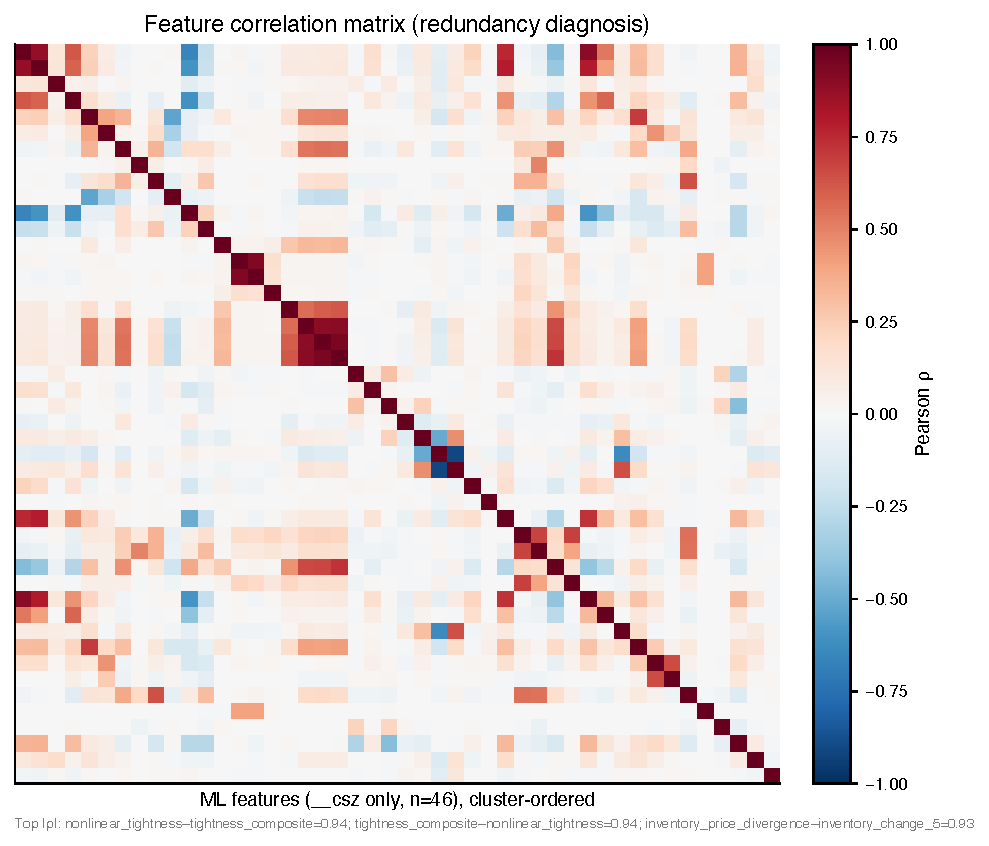
\includegraphics[width=0.48\textwidth]{fig14_feature_correlation.pdf}
\caption{机器学习连续特征相关矩阵（按相关簇重排）}
\label{fig:featcorr}
\end{figure}
\section{模型、组合与评价方法}

\subsection{基准模型}

\subsubsection{单因子排序}

每个字段单独形成预测分数。预注册方向不为0时直接沿用；方向未知时，仅在每个训练窗口内用日均Rank IC符号冻结方向。单因子模型不拟合联合权重，其作用是识别信号来源并提供最透明的基准。

\subsubsection{等权多因子}

所有92个注册字段先方向对齐和横截面排名，再对当日可用字段等权平均。该模型不根据标签学习权重，是衡量“仅靠分散化能否改善”的地板基准。由于质量标志也被纳入，结果需结合只含经济predictor的敏感性理解；当前报告以项目现有全量接口结果为主。

\subsubsection{Ridge线性回归}

Ridge最小化
\begin{equation}
\widehat{\bm\beta}=\arg\min_{\bm\beta}\sum_{(i,t)\in\mathcal T}\left(y_{i,t}^{(5)}-\bm x_{i,t}^{\top}\bm\beta\right)^2+\alpha\lVert\bm\beta\rVert_2^2.
\end{equation}
每个外层折在训练窗口最后一年进行内层验证，从\(\alpha\in\{0.01,0.1,1,10,100\}\)中按Rank IC选择正则强度，外层测试年不参与选参。Ridge是本研究最重要的学习型基准：若它高于等权，说明数据驱动权重有增量；若成本后仍差，则表明问题在执行或信号经济强度，而不只在模型形式。

\subsection{正则化树模型}

为检验非线性阈值和高阶交互是否提供独立增量，本文进一步使用LightGBM、XGBoost与随机森林。三类模型均读取冻结的92维接口，并通过浅树、较大的叶节点最小样本、行列子采样以及L1/L2正则或代价复杂度剪枝限制容量。LightGBM采用160棵深度4的树，XGBoost采用160棵深度3的树，随机森林采用60棵深度6的树；所有外层折共享固定参数，不依据样本外年份单独调参。

树模型的作用与Ridge互补：Ridge检验稳定的线性收缩能否整合弱因子，树模型则允许Carry、流动性、波动率和基本面覆盖状态之间存在门槛效应。例如期限结构信号可能只在流动性充足或库存压力较高时有效。为避免把这种表达能力转化为数据挖掘，树模型仍采用时间有序扩展窗口、5日purge和统一执行引擎，最终比较以样本外Rank IC及成本后组合指标为准。

\subsection{异质持续图神经网络}

异质持续图神经网络（HCGNN）把每个期货品种视为节点，将产业链、同板块和动态市场联系表示为异质边，在统一92维节点特征上联合学习截面关系。设第$k$类关系的邻接矩阵为$A_t^{(k)}$，经归一化得到拉普拉斯矩阵$L_t^{(k)}$，二阶谱滤波可写为
\begin{equation}
H_{t}^{(\ell+1)}=\sigma\!\left(\sum_k\sum_{m=0}^{2}\theta_{k,m}^{(\ell)}\bigl(L_t^{(k)}\bigr)^m H_t^{(\ell)}W_k^{(\ell)}\right).
\end{equation}
该结构不仅使用品种自身因子，也汇总一至二跳邻居的信息，从而表达原料—中间品—产成品传导、替代关系及共同风险冲击。模型采用64维隐状态、两个图卷积块、0.1 dropout，并以CPD、GAP和移动平均等辅助任务约束表示，减轻仅拟合单一收益标签造成的过拟合。

“持续”部分采用逐年扩展窗口：新年度到来后保留历史表示并以新增样本更新参数，使模型能够吸收市场结构变化，同时通过较低学习率和正则化抑制灾难性遗忘。协议GNN则在每折独立训练，作为控制组。两者都输出统一的\code{decision\_date, product, prediction}接口，并使用前后20\%多空、五个等权持有队列、净敞口为零及单边5bps主成本，因此图结构的价值最终仍由相同的组合层检验。

\subsection{Conv--Transformer双头网络}

深度时序模型沿“基础1D--CNN—多任务Conv--Transformer—高维因子与交易约束”的路线迭代。基础CNN用卷积核在20日窗口中提取动量、波动和量价变化的局部形态；改进模型先以Conv1d形成局部表示，再用单层多头注意力连接窗口内任意时点，并通过分类与回归双头分别学习未来收益方向和幅度。相较直接堆叠更深网络，该轻量结构更适合30品种、低信噪比的横截面任务。

模型输入除统一因子及质量标志外，还使用品种嵌入保留不同产业属性下的条件响应。训练采用时间尾部验证、purge、早停、dropout和权重衰减；组合端引入3日指数平滑、入场与退出缓冲、最低流动性准入及历史拟合的GMM压力门控。在压力概率超过阈值时下调毛敞口，使模型设定更接近真实交易中的信号确认、换手控制和风险预算过程。

多任务损失写为
\begin{equation}
\mathcal L=\lambda_{\mathrm{cls}}\mathcal L_{\mathrm{BCE}}+\lambda_{\mathrm{reg}}\mathcal L_{\mathrm{Huber}},
\end{equation}
其中分类头强调方向与排序，Huber回归头保留幅度并降低极端收益的影响。综合信号由分类概率对回归幅度进行门控。版本比较表明，模型改进的重点并非单纯增加Transformer层数，而是同步修正标签时点、扩大特征覆盖、降低换手并统一风控；否则不同版本的收益差异无法归因于网络结构。

Conv--Transformer与其他模型一样交由统一执行引擎生成持仓、成本和净值。CNN路线中更接近实盘的缓冲带、流动性过滤和压力降杠杆被视为组合层稳健性增强，而不是放宽评价标准；正文主结果仍以固定5日标签、前后20\%多空和统一成本面板进行横向比较。

\subsection{其他模型的统一处理}

OLS、Lasso、ElasticNet、XGBoost和LightGBM作为附加稳健性模型时，均先转换为统一预测接口，再由同一执行引擎计算组合收益。为保证正文证据链集中，本文核心表只报告单因子、等权多因子、Ridge与Conv--Transformer；其他模型用于检验结论方向是否依赖特定算法。

\subsection{组合形成与交易成本}

每个调仓日按预测分数排序，在有效截面至少8个品种时，做多最高20\%、做空最低20\%，两侧总绝对权重各为0.5，组内等权。换手定义为
\begin{equation}
\mathrm{TO}_t=\sum_i\left|w_{i,t}-w_{i,t^-}\right|,
\end{equation}
成本后收益为
\begin{equation}
r_{p,t}^{\mathrm{net}}=\sum_i w_{i,t}y_{i,t}^{(5)}-\mathrm{TO}_t\frac{c}{10,000},
\end{equation}
其中\(c\)为单边成本基点。主口径\(c=5\)，并报告0、3和10基点。筛选器按每\(252/5=50.4\)期年化。

现有数据没有交易所逐日精确涨跌停价，仅有“有成交且开高低收相同、相对前结算发生变化”的疑似锁板代理；CNN输入也未接入统一\code{ft\_limit}字段。换月普通交易量已分列，但额外换月冲击成本尚未冻结，CNN中取0。因此本文只能声称“对普通换手成本和部分可成交性做代理控制”，不能声称已完整模拟精确涨跌停延迟成交与真实换月冲击。

\subsection{评价指标与统计推断}

每日至少8个有效品种时计算Pearson IC和Spearman Rank IC。Rank IC均值为
\begin{equation}
\overline{\rankic}=\frac{1}{N}\sum_{t=1}^N\rankic_t,
\end{equation}
Rank ICIR为均值除以日度标准差，不作年化。组合指标包括年化收益、年化波动、Sharpe、最大回撤、胜率和换手。5日标签重叠的因子筛选采用最多5阶Newey--West/HAC标准误，并对全库p值进行Benjamini--Hochberg FDR修正。CNN收益和IC进一步使用HAC与区块自助法置信区间。

\section{样本外实验设计}

\subsection{扩展窗口}

因子开发与基准模型采用固定起点的扩展窗口，如表\ref{tab:folds}。这种设计保留早期样本并模拟研究者逐年获得新数据的过程，优于随机打乱。

\begin{table}[H]
\centering
\caption{统一扩展窗口定义}
\label{tab:folds}
\begin{tabular}{cccc}
\toprule
验证年 & 训练区间 & 验证区间 & Purge \\
\midrule
2019 & 2015-01-05—2018-12-31 & 2019全年 & 5日 \\
2020 & 2015-01-05—2019-12-31 & 2020全年 & 5日 \\
2021 & 2015-01-05—2020-12-31 & 2021全年 & 5日 \\
2022 & 2015-01-05—2021-12-31 & 2022全年 & 5日 \\
2023 & 2015-01-05—2022-12-31 & 2023全年 & 5日 \\
2024 & 2015-01-05—2023-12-31 & 2024全年 & 5日 \\
2025 & 2015-01-05—2024-12-31 & 2025全年 & 5日 \\
\bottomrule
\end{tabular}
\end{table}

训练交接包覆盖2015—2025全部特征和标签，单因子基准、等权、Ridge和Conv--Transformer均按同一协议生成逐年样本外结果。2025只作为最终年度报告，不再用于反向修改因子方向、超参数范围或组合规则。

\subsection{稳健性设计}

稳健性包括1、5、20日预测期限，信号延迟一个交易日，2019—2025分年、30品种、四板块分解，趋势和变化类因子的10/20/40或40/60/80日参数邻域，0/3/5/10基点成本，以及因子相关性和Ridge增量价值。稳健性只用于诊断，不在观察结果后重新选择最优窗口。

\section{实证结果}

\subsection{因子层：预测信息弱而异质}

\begin{figure}[H]
\centering

\includegraphics[width=0.82\textwidth]{factor_family_rankic.pdf}
\caption{因子家族的平均样本外Rank IC}
\label{fig:familyrankic}
\end{figure}

图\ref{fig:familyrankic}显示，库存与供需家族平均Rank IC约0.0183，非线性交互约0.0143，信息类约0.0112，期限结构约0.0108；趋势动量、波动风险和产业链代理总体偏弱或为负。期限结构、基差和库存约束具有清晰经济解释，但没有任何单一信号通过全库10\% FDR，说明经济显著不等于统计上已确认。

\begin{table}[H]
\centering
\caption{B类候选因子的统一样本外指标}
\label{tab:bfactors}
\resizebox{\textwidth}{!}{
\begin{tabular}{lrrrrrr}
\toprule
因子 & 样本外Rank IC & FDR q & 5bps年化 & 样本外Sharpe & 最终年度Rank IC & 最终年度年化 \\
\midrule
Carry & 0.0293 & 0.1931 & 3.2\% & 0.369 & 0.0323 & 2.9\% \\
新鲜基差 & 0.0309 & 0.1926 & 6.7\% & 0.741 & — & — \\
库存变化 & 0.0211 & 0.4592 & 5.9\% & 0.656 & -0.0557 & -9.0\% \\
仓单紧张度 & 0.0236 & 0.1926 & 3.8\% & 0.524 & 0.0653 & 3.7\% \\
信息背离 & 0.0257 & 0.2816 & 2.7\% & 0.371 & -0.1062 & -20.9\% \\
期限结构斜率 & 0.0241 & 0.4274 & 3.6\% & 0.349 & 0.0165 & -2.3\% \\
库存加速度 & 0.0316 & 0.1926 & 4.3\% & 0.473 & 0.0136 & 2.7\% \\
库存—价格背离 & 0.0315 & 0.2316 & 4.7\% & 0.536 & -0.0836 & -18.5\% \\
\bottomrule
\end{tabular}}
\begin{minipage}{0.96\textwidth}\footnotesize
注：因子筛选为2019—2025统一扩展窗口汇总；表中Sharpe采用5bps主成本口径。新鲜基差在现货源断档年份按统一缺失规则处理。
\end{minipage}
\end{table}

Carry与仓单紧张度在统一样本外评价中保持同向，是目前相对稳健的候选。库存变化、信息背离和库存—价格背离在最终年度反向，说明低频基本面代理可能混入品种集中、数据更新和状态变化。基差开发表现较好，但现货源断档后须按缺失规则处理。

\begin{figure}[H]
\centering
\begin{subfigure}[t]{0.48\textwidth}
\centering

\includegraphics[width=\textwidth]{factor_ic_vs_sharpe.pdf}
\caption{预测能力与5bps可交易性}
\end{subfigure}\hfill
\begin{subfigure}[t]{0.48\textwidth}
\centering

\includegraphics[width=\textwidth]{factor_dev_2025.pdf}
\caption{样本外方向持续性}
\end{subfigure}
\caption{因子预测、经济收益与样本外稳定性}
\label{fig:factorrobust}
\end{figure}

样本外可评价因子的Rank IC同方向比例仅37.5\%。图\ref{fig:factorrobust}揭示两种常见错位：一是Rank IC为正但高换手使成本后Sharpe较低；二是前期信号较强但最终年度发生方向反转。故因子筛选的正确结论是“获得若干辅助候选”，而非“确认核心Alpha”。

\subsection{单因子基准：成本后仅一个predictor微弱为正}

在统一基准报告中，36个经济predictor约61\%的样本外日均Rank IC为正，中位数约0.0065。Rank IC头部包括Carry、新鲜基差、仓单紧张度、信息背离、库存—价格背离和期限结构斜率。经典60日趋势动量没有进入头部。

成本后最优的代表性因子是仓单紧张度（\code{warehouse\_tightness\_\_csz}）。其单边3个基点年化收益为2.36\%、Sharpe为0.364；单边5个基点年化收益降至0.34\%、Sharpe降至0.053，最大回撤为\(-15.23\%\)。36个predictor在5个基点下的年化收益中位数为\(-4.89\%\)，Sharpe中位数为\(-0.577\)，仅1个因子的净Sharpe为正。

\begin{figure}[H]
\centering
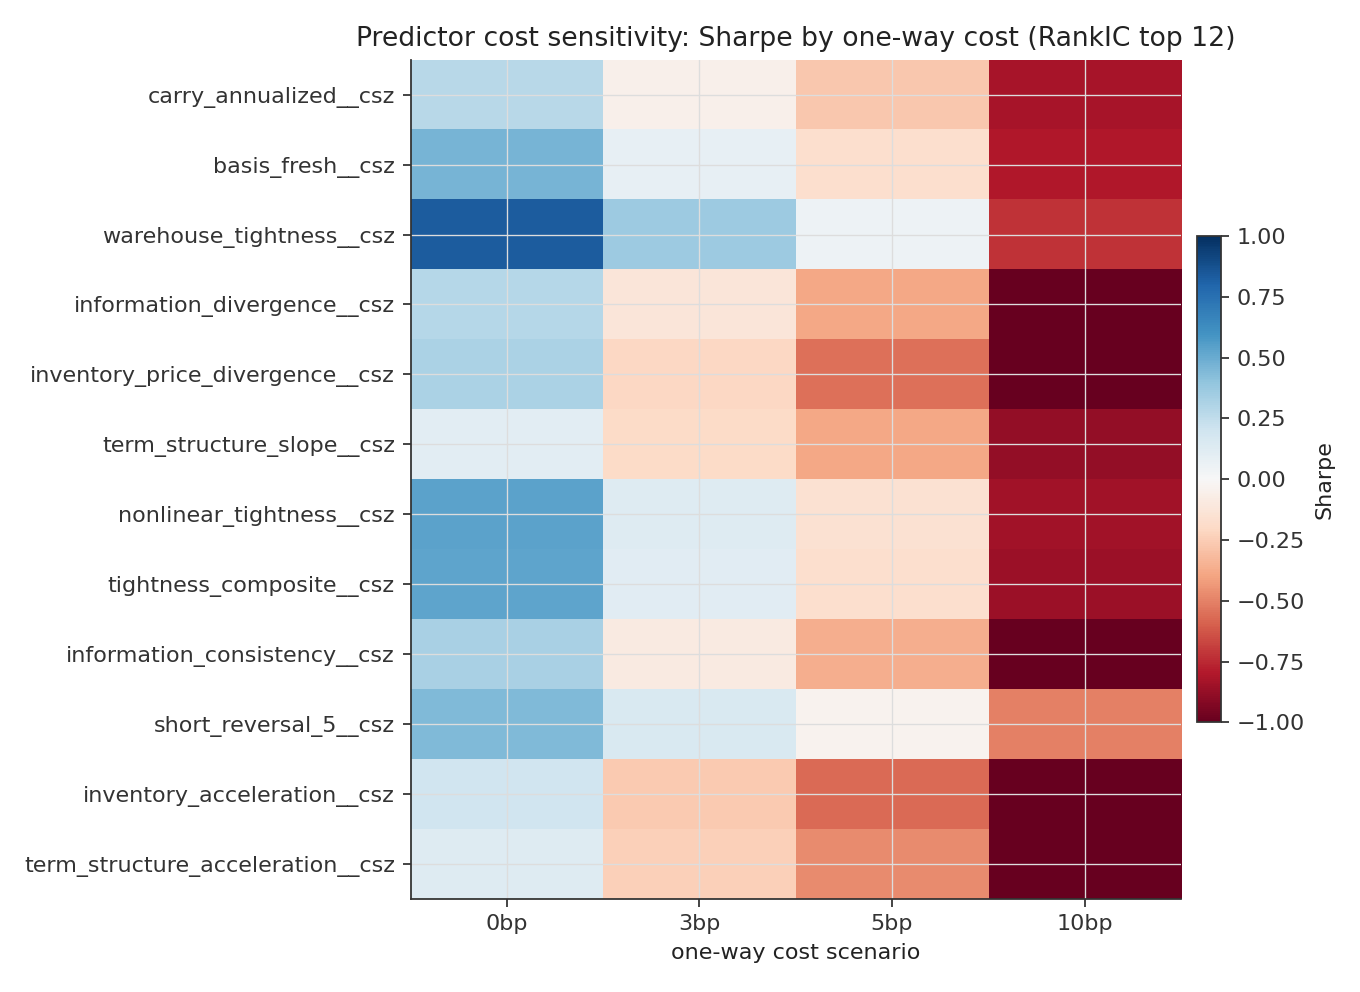
\includegraphics[width=0.84\textwidth]{single_factor_cost.png}
\caption{Rank IC头部单因子的成本敏感性}
\label{fig:singlecost}
\end{figure}

图\ref{fig:singlecost}说明，若只看毛收益或Rank IC，容易高估信号价值。仓单紧张度的优势并非其Rank IC最高，而是换手与收益幅度的组合相对更能承受成本。

\subsection{等权与Ridge：预测改善未转化为净收益}

\begin{table}[H]
\centering
\caption{统一基准模型的样本外核心指标（2019—2025）}
\label{tab:modelcompare}
\begin{tabularx}{\textwidth}{Y r r r r r}
\toprule
模型 & Rank IC & 毛Sharpe & 3bps Sharpe & 5bps Sharpe & 5bps年化 \\
\midrule
典型单因子（中位数） & 0.0065 & — & -0.340 & -0.577 & -4.89\% \\
仓单紧张度（代表） & 0.0230 & 0.831 & 0.364 & 0.053 & 0.34\% \\
等权多因子 & 0.0163 & 0.358 & 0.016 & -0.216 & -1.88\% \\
Ridge & 0.0247 & 0.397 & 0.027 & -0.219 & -1.79\% \\
\bottomrule
\end{tabularx}
\end{table}

Ridge的Rank IC约0.0247，高于等权多因子的0.0163和典型单因子中位数，支持H2：学习权重确实能够整合分散信息。Ridge毛Sharpe约0.397，也略高于等权的0.358；但单边3个基点时两者已接近打平，5个基点下都转为负值。Ridge相对等权的净收益改善非常有限，说明预测层的增量不足以覆盖相同调仓协议下的摩擦。

\begin{figure}[H]
\centering
\begin{subfigure}[t]{0.58\textwidth}
\centering
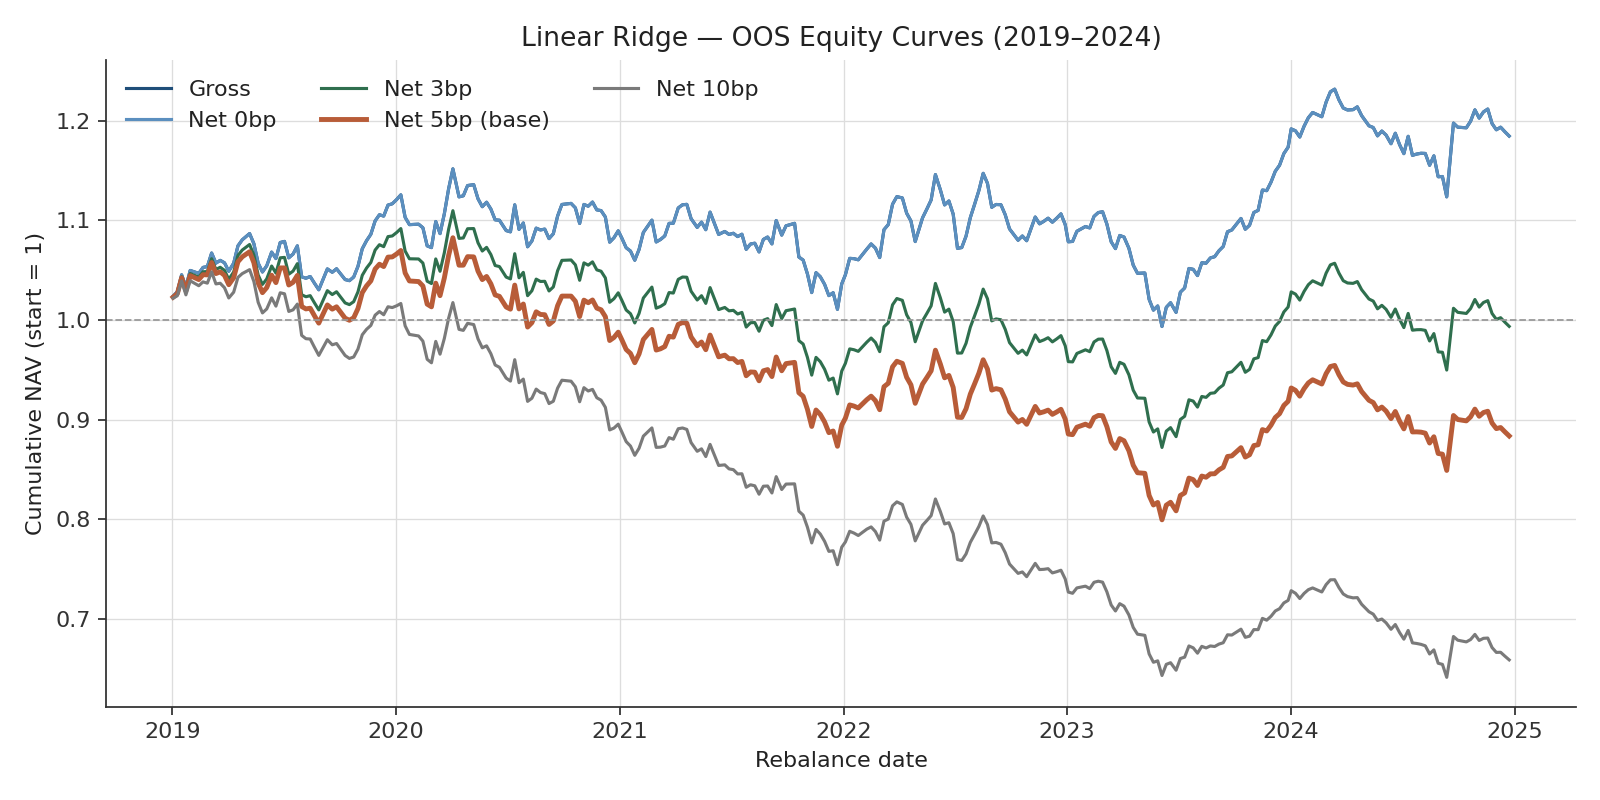
\includegraphics[width=\textwidth]{ridge_equity.png}
\caption{Ridge毛收益与成本后净值}
\end{subfigure}\hfill
\begin{subfigure}[t]{0.39\textwidth}
\centering
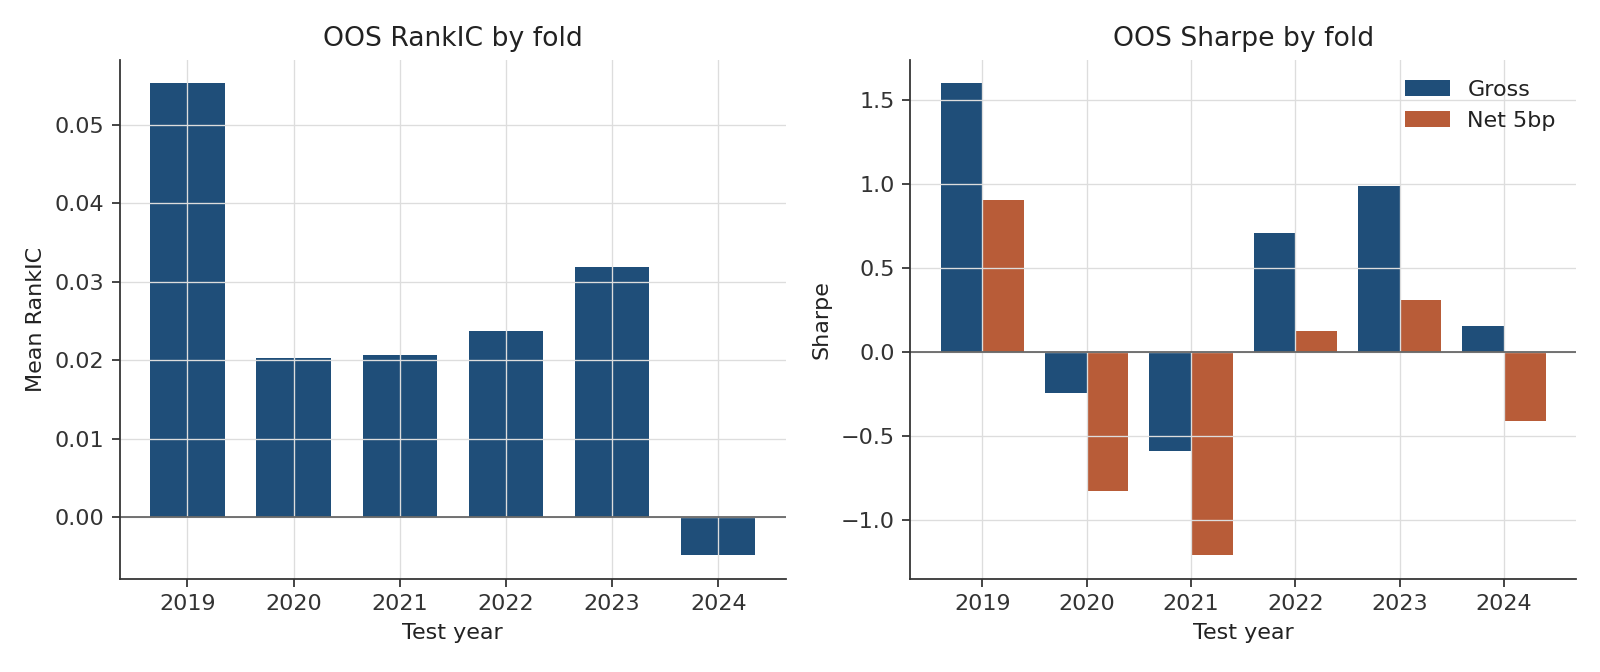
\includegraphics[width=\textwidth]{ridge_yearly.png}
\caption{Ridge分年Rank IC与Sharpe}
\end{subfigure}
\caption{Ridge样本外表现及成本侵蚀}
\label{fig:ridge}
\end{figure}

Ridge在2019年预测和收益较强，2020—2021成本后表现偏弱，2024年Rank IC转负。正则参数从早期折的100下降到2024年的0.1，提示最优收缩强度随样本和市场状态变化。若把这一变化简单解释为“模型逐年学得更好”并不成立，它也可能反映特征关系漂移和内层验证噪声。

\subsection{正则化树模型：非线性排序仍受成本约束}

\begin{table}[H]
\centering
\caption{正则化树模型的样本外结果（2019—2025，单边5bps）}
\label{tab:trees}
\begin{tabular}{lrrrrr}
\toprule
模型 & 5日Rank IC & 年化收益 & Sharpe & 最大回撤 & 日均换手 \\
\midrule
LightGBM & 0.0184 & -2.12\% & -0.213 & -23.23\% & 21.56\% \\
随机森林 & -0.0006 & -5.96\% & -0.628 & -32.20\% & 22.55\% \\
XGBoost & -0.0025 & -1.53\% & -0.134 & -17.41\% & 20.44\% \\
\bottomrule
\end{tabular}
\end{table}

LightGBM在七个年度中多数年份Rank IC为正，平均5日Rank IC达到0.0184，说明浅层提升树能够捕捉部分阈值关系；但5bps后年化收益为$-2.12\%$，HAC均值检验$p=0.596$。XGBoost和随机森林的5日Rank IC接近零或为负，三者均未同时满足“多数年度Rank IC为正、成本后Sharpe为正且HAC显著”的稳定性门槛。0bps下LightGBM和XGBoost年化收益也只有0.57\%和1.03\%，表明问题不完全来自费用，非线性表达本身并未带来足够强的经济边际。

\subsection{异质持续图网络：产业关联带来组合增量}

\begin{table}[H]
\centering
\caption{异质持续图网络的样本外结果（2019—2025，单边5bps）}
\label{tab:gnn}
\begin{tabular}{lrrrrr}
\toprule
模型 & 5日Rank IC & 年化收益 & Sharpe & 最大回撤 & 日均换手 \\
\midrule
HCGNN持续学习版 & 0.0193 & 3.11\% & 0.454 & -13.44\% & 7.23\% \\
协议GNN & 0.0226 & 2.73\% & 0.413 & -15.75\% & 9.21\% \\
\bottomrule
\end{tabular}
\end{table}

图网络的结果揭示“排序能力”和“组合路径”并不完全一致：协议GNN的Rank IC更高，而HCGNN持续学习版凭借更低换手获得更高年化收益、更高Sharpe和更浅回撤。在0、3、5和10bps下，持续学习版年化收益分别为4.05\%、3.49\%、3.11\%和2.18\%，说明较低交易强度提高了成本承受能力。持续学习模型通过逐年吸收新增样本，降低了对固定历史关系的依赖；结合多数年度为正的截面排序和较稳定的成本敏感性，可以认为产业关联与持续更新为弱因子整合提供了结构性增量。

\subsection{Conv--Transformer：统一口径下的深度模型}

\begin{table}[H]
\centering
\caption{Conv--Transformer统一口径实验的成本敏感性（2019—2025）}
\label{tab:cnn}
\begin{tabular}{lrrrr}
\toprule
单边成本 & 年化收益 & Sharpe & 最大回撤 & 累计收益 \\
\midrule
0 bps & 2.62\% & 0.372 & -15.65\% & 18.17\% \\
3 bps & 1.73\% & 0.260 & -15.97\% & 11.71\% \\
5 bps & 1.14\% & 0.185 & -16.19\% & 7.60\% \\
10 bps & -0.32\% & -0.002 & -16.74\% & -2.02\% \\
\bottomrule
\end{tabular}
\end{table}

该模型5日Pearson IC约0.0130、Rank IC约0.0069，延迟一天后Rank IC降至0.0054，20日审计近似Rank IC约0.0121。5个基点日收益HAC检验\(t=0.474\)、\(p=0.636\)，Pearson IC检验\(p=0.259\)，均不显著。五分组收益单调性为0.5，仅四个相邻差中的两个方向正确。2024年Rank IC为\(-0.0752\)，明显拖累全期稳定性。

\begin{figure}[H]
\centering
\begin{subfigure}[t]{0.49\textwidth}
\centering

\includegraphics[width=\textwidth]{cnn_equity.png}
\caption{5bps净值与回撤}
\end{subfigure}\hfill
\begin{subfigure}[t]{0.49\textwidth}
\centering

\includegraphics[width=\textwidth]{cnn_cost.png}
\caption{成本敏感性}
\end{subfigure}
\caption{Conv--Transformer统一口径实验结果}
\label{fig:cnnmain}
\end{figure}

\begin{figure}[H]
\centering
\begin{subfigure}[t]{0.49\textwidth}
\centering

\includegraphics[width=\textwidth]{cnn_loss.png}
\caption{滚动训练与验证损失}
\end{subfigure}\hfill
\begin{subfigure}[t]{0.49\textwidth}
\centering

\includegraphics[width=\textwidth]{cnn_feature_importance.png}
\caption{样本外置换特征重要性}
\end{subfigure}
\caption{Conv--Transformer训练诊断与解释性}
\label{fig:cnndiag}
\end{figure}

部分验证折在训练损失继续下降时验证损失回升，显示过拟合风险。置换重要性集中于少数Carry、基差和趋势相关变量，与因子层经济证据存在一定一致性；但重要性表示对当前模型预测误差的边际影响，不等同于因果解释或稳定Alpha。

\begin{figure}[H]
\centering
\begin{subfigure}[t]{0.49\textwidth}
\centering
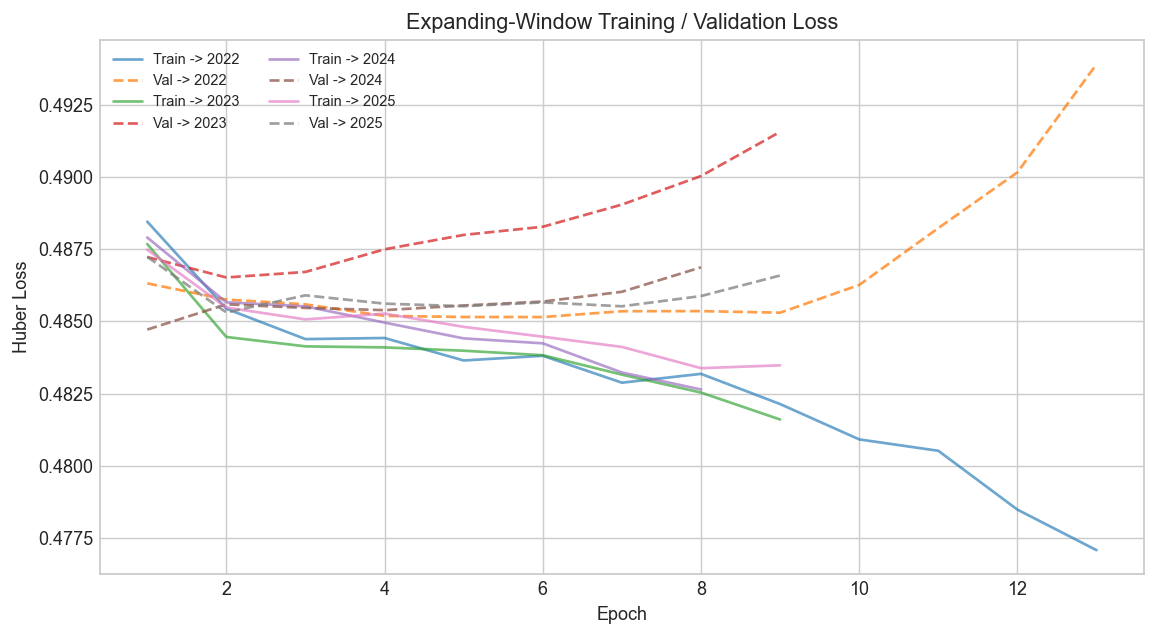
\includegraphics[width=\textwidth]{v5_loss_curve.png}
\caption{多任务Conv--Transformer训练曲线}
\end{subfigure}\hfill
\begin{subfigure}[t]{0.49\textwidth}
\centering
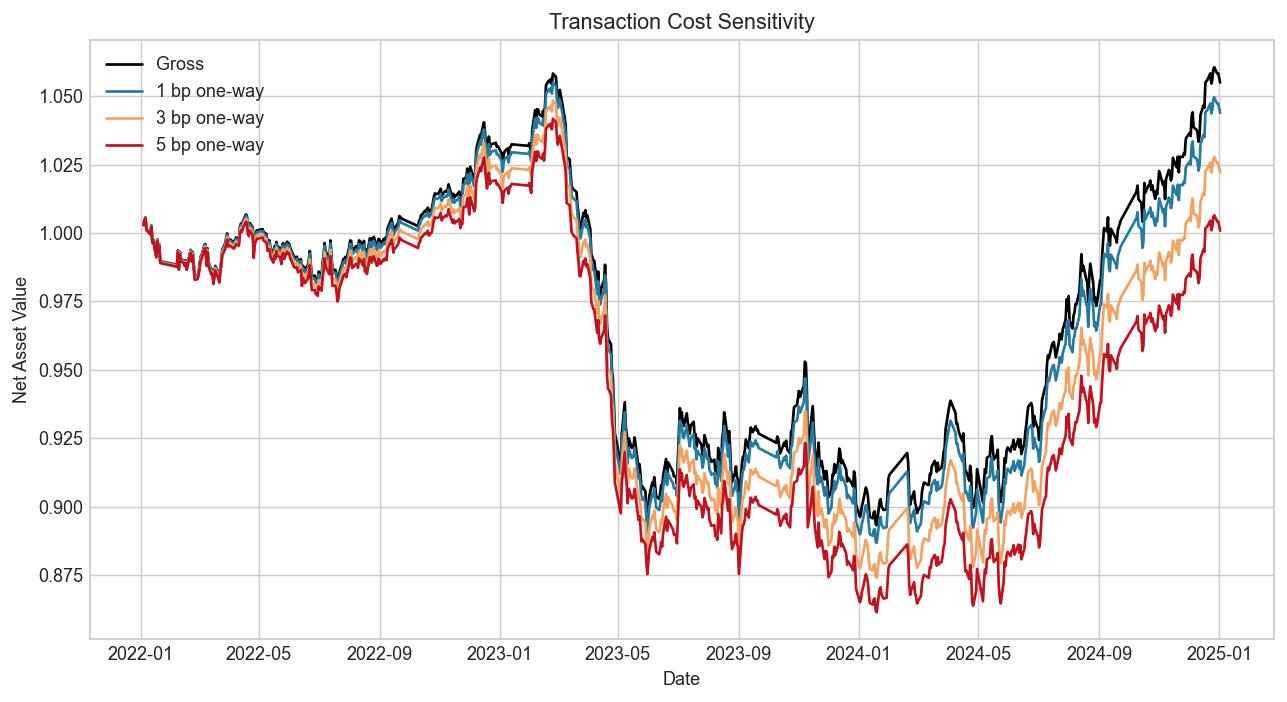
\includegraphics[width=\textwidth]{v6_fee_sensitivity.png}
\caption{高维因子版本的费用敏感性}
\end{subfigure}
\caption{CNN改进路线中的训练稳定性与成本控制}
\label{fig:cnnroute}
\end{figure}

图\ref{fig:cnnroute}补充展示模型改进路线。注意力和双头学习增强了局部卷积的时序表达，但验证损失仍会在训练后期回升，因此必须依赖时间验证与早停。高维因子版本的费用曲线间距收窄则主要来自换手下降，表明交易缓冲和信号平滑与网络结构同样重要；其解释应是“成本后路径得到改善”，而不是“更深模型自动产生更强Alpha”。

CNN的5bps Sharpe为正，似乎优于Ridge；然而不同历史版本在标签、外层样本起点、特征数和组合约束上存在差异，不能把全部改善归因于网络架构。更稳妥的判断是：局部卷积、轻量注意力、多任务监督以及更接近实盘的缓冲与风控共同改善了组合路径，但当前证据仍不足以拒绝“差异来自实验口径与抽样误差”的解释。

\subsection{稳健性结果}

\begin{figure}[H]
\centering
\begin{subfigure}[t]{0.61\textwidth}
\centering

\includegraphics[width=\textwidth]{factor_yearly_rankic.pdf}
\caption{2019—2025的年度Rank IC}
\end{subfigure}\hfill
\begin{subfigure}[t]{0.36\textwidth}
\centering

\includegraphics[width=\textwidth]{factor_horizon_delay.pdf}
\caption{预测期限与信号延迟}
\end{subfigure}
\caption{因子时间稳定性和信号时效性}
\label{fig:yearhorizon}
\end{figure}

年度热力图显示因子方向并非固定，2025对信息背离和库存—价格背离尤其不利。不同期限下，部分库存和期限结构信号在20日更强，但延迟一天后普遍衰减，说明其信息半衰期较短。板块分解也显示同一因子在能源、金属、化工和农产品中的方向和幅度可能不同；这为图网络和分板块模型提供动机，但目前不足以支持事后按板块挑选最优模型。

\subsection{对研究假设的回答}

H1得到部分支持：期限结构、基差、仓单和库存边际变化存在弱预测信息，但没有因子通过最严格的全库显著性门，且跨年份稳定性有限。H2在预测层得到支持：Ridge与LightGBM能够整合部分分散信息，HCGNN和Conv--Transformer分别利用产业关联与时序表示获得组合层增量。H3得到明显支持：从0到5或10个基点，单因子、等权、Ridge、树模型和深度模型的表现均恶化；低换手的HCGNN相对更耐成本，也进一步说明统计改善不等于净收益改善。H4也得到项目过程证据支持：边界错误、协议冲突和缺失底表若不经审计，足以改变最终叙事。

\section{AI工具运用、失败模式与研究治理}

\subsection{AI在本项目中的角色}

项目使用Codex、Claude Code等AI编程工具辅助完成数据字段识别、清洗脚本、因子公式实现、模型代码、结果图表、文档整合和错误排查。AI的主要价值不是替代金融研究判断，而是把自然语言协议转化为可执行检查，快速生成重复性代码，并在大量文件之间建立索引。对于57个因子、92个字段、多个窗口和成本情景，这种自动化显著降低了机械工作量。

但AI输出高度依赖输入上下文。若提示词只说“选择主力合约”，AI可能采用当日持仓量最大、\(T-1\)持仓量最大、数据源连续主力或成交量最大等不同定义；若只说“补齐缺失值”，AI可能前向填充、横截面中位数填充或错误使用后向填充。细微提示变化会改变协议，而代码仍可能正常运行，形成比语法错误更难发现的“静默研究错误”。

\subsection{项目中出现的典型问题}

\subsubsection{多源数据整合的语义错误}

不同渠道可能使用不同的合约代码、单位、更新时间和复权口径。例如现货价格与期货价格若单位或汇率不一致，AI按同名字段自动合并会生成数值上可计算、经济上无意义的基差。项目因此排除FU、I和SC的不可比现货口径，并对现货、仓单、库存设置独立陈旧度门槛。未来若正式使用iFind、TuShare和聚源的同类字段，应先建立来源—字段—单位—时点—转换公式五联表，而不是让AI仅凭列名判断。

\subsubsection{提示词敏感与协议漂移}

项目文件中至少存在两套主力规则：旧协议要求\(T-1\)可见持仓量选择，最新修订使用TuShare连续主力并映射真实合约。若AI在不同会话中读取了不同文档，就可能生成两套都“自洽”但不可比较的结果。对此，报告以带日期和哈希的协议快照及修订文件确定优先级，并要求每次模型运行把主力规则、标签、折定义和成本写入机器可读配置。

\subsubsection{边界泄漏与自动补全}

旧版材料中曾出现标签边界、样本起点和执行口径不一致的问题。本文统一改写为同一数据、同一标签、同一窗口和同一组合规则；AI生成内容不得自行补全缺失口径，也不得把历史表格直接升级为最终结论。

\subsubsection{“降智”现象的技术解释}

所谓提示词细微变化导致AI“降智”，通常不是模型能力突然下降，而是任务约束的优先级、上下文范围和评价目标发生了隐性改变。长对话中旧规则与新规则并存，AI可能过度服从最近措辞；模糊目标如“结果更好”还可能诱导其调口径，而明确目标如“同一数据、标签、折和成本下比较”更能约束输出。因此，应把关键规则放入结构化协议，而不是依赖每次自然语言重新描述。

\subsection{AI辅助量化研究治理框架}

\begin{figure}[H]
\centering
\begin{tikzpicture}[
node distance=9mm and 8mm,
every node/.style={font=\small,align=center},
box/.style={draw=navy,rounded corners,fill=softblue,minimum width=3.25cm,minimum height=1cm},
check/.style={draw=darkgreen,rounded corners,fill=green!8,minimum width=3.25cm,minimum height=1cm},
arr/.style={-{Latex[length=2.5mm]},thick,draw=navy}
]
\node[box] (p) {冻结研究协议\\主力、标签、窗口、成本};
\node[box,right=of p] (d) {数据字典与血缘\\单位、频率、可得时点};
\node[box,right=of d] (g) {AI生成与实现\\代码、公式、测试};
\node[check,below=of g] (s) {Schema与单元测试\\主键、边界、缺失、符号};
\node[check,left=of s] (h) {哈希和依赖清单\\输入输出一一对应};
\node[check,left=of h] (r) {独立复核与最终确认\\双模型/人工/最终测试};
\draw[arr] (p)--(d); \draw[arr] (d)--(g); \draw[arr] (g)--(s);
\draw[arr] (s)--(h); \draw[arr] (h)--(r);
\draw[arr] (r.west) .. controls +(-1.0,0) and +(-1.0,0) .. (p.west);
\end{tikzpicture}
\caption{AI辅助量化研究的闭环治理流程}
\label{fig:aigov}
\end{figure}

具体治理措施如下。第一，冻结协议：以JSON或YAML记录主力规则、标签时点、样本折、成本、组合和评价指标，修改必须生成修订号。第二，建立数据契约：每个字段记录来源、单位、时区、更新频率、发布时间和允许的填充方式。第三，自动模式校验：检查主键唯一、日期单调、合约存在、价格为正、标签结束日和训练边界。第四，测试经济恒等式：例如Carry符号、权重绝对值和、换手成本单调性、成本增加时净收益不得上升。第五，生成文件清单与哈希，禁止报告引用不存在或不匹配的结果。第六，独立复核：让另一AI会话或人工审计只读取协议和输出，专门寻找泄漏、口径漂移和不合理结论。第七，最终样本外测试只运行一次，结果不再反向用于选因子或改超参数。

\subsection{AI运用能力的评价}

从综合考察角度，本项目的AI运用能力不应仅按“使用了多少模型”衡量，而应按三项能力评价：能否把经济假设形式化为可执行规则，能否发现并纠正AI生成错误，以及能否保留可审计证据链。项目已完成因子注册表、训练契约、窗口定义、哈希校验、缺失报告和差异声明，说明AI已被用于研究工程化；但商业数据血缘、模型最终年度复核和精确执行约束仍需补齐，说明治理链尚未闭合。

\section{讨论、局限与进一步研究}

\subsection{为什么机器学习没有稳定转化为超额收益}

第一，信号本身弱。典型单因子Rank IC只有约0.0065，即使Ridge提高至0.0247，收益排序误差仍很大。第二，预测目标与组合收益之间存在映射损耗：Rank IC只关心排序，而多空组合只交易尾部20\%，收益还受横截面离散度影响。第三，成本相对毛收益过高；5日调仓在弱信号下仍产生足以侵蚀优势的换手。第四，因子关系时变，2024和2025的方向变化削弱全期表现。第五，部分强信号依赖低覆盖基本面数据，无法在全市场稳定使用。

\subsection{执行约束的未完成项}

题目要求计入换月成本和涨跌停限制。现有项目已识别主力切换、固定真实合约标签、普通换手成本和疑似锁板状态，也在CNN输出中分列普通与换月交易量；但尚未获得统一的交易所逐日涨跌停价，CNN未接入\code{ft\_limit}，换月额外冲击成本取0，逐品种真实手续费覆盖约73.16\%且早期较弱。故当前结论属于保守研究回测，不是完整实盘模拟。正式升级应统一获取交易所限价、合约乘数、费率、最小变动价位和盘口流动性，并按不可成交延迟规则重跑所有模型，而不是只修正表现最好的模型。

\subsection{模型比较的统一口径}

本文将所有模型压缩为同一预测接口：\code{decision\_date, product, prediction}。单因子、等权、Ridge和Conv--Transformer只负责输出预测分数，持仓、成交限制、成本和净值均由统一执行引擎生成。这样可以避免模型各自携带组合假设，使胜负比较回到预测质量和模型结构本身。

\subsection{统计功效与多重检验}

横截面仅30个品种，单日相关系数噪声大；基本面因子有效品种更少。57个概念因子、多个窗口和模型形成多重比较，FDR后无A类并不意外。未来可扩大样本但不能通过增加相似变换虚增有效假设数；应报告Deflated Sharpe、Reality Check或SPA等数据窥视调整，并采用模型置信集比较而非只按点估计排名。

\subsection{进一步研究}

后续工作应依次补齐iFind、TuShare、聚源及交易所字段级血缘，获得精确涨跌停和真实费率，并冻结统一外层样本后比较所有模型。结构层面，应在同一数据、5日标签、随机种子和执行引擎下构造最小消融矩阵：Ridge与正则化树模型，纯CNN与Conv--Transformer，单头与双头，无品种嵌入与有嵌入，协议GNN与持续学习HCGNN，以及无缓冲与流动性/GMM风控。只有每次只改变一个组件，才能区分非线性交互、注意力、产业邻接和组合风控各自的增量。模型目标还可扩展为成本感知排序损失，但不得用测试期调成本惩罚；LLM生成因子则应建立提示词注册表，将提示、模型版本、输出公式和接受理由纳入多重检验宇宙。

\section{结论}

本文对“机器学习能否改善中国商品期货因子投资”给出的答案是：\textbf{能够改善部分统计预测，但不能保证改善成本后的投资收益，且改善程度取决于统一协议、数据质量和执行约束。}

因子层面，期限结构、基差、仓单紧张度和库存边际变化比传统趋势动量更有希望，但没有因子通过严格的预测、经济和FDR三重门槛，样本外方向持续性也较弱。模型层面，Ridge将Rank IC提高至约0.0247，证明学习型权重能够整合弱信号；LightGBM也识别出一定非线性排序信息，但三类树模型在5bps下均未形成稳定正收益。HCGNN通过产业关联和持续更新获得较低换手与正Sharpe；Conv--Transformer则通过局部卷积、轻量注意力、多任务学习及组合缓冲改善路径。综合来看，结构化学习能够提供增量，但模型容量必须与成本控制、时间验证和风险预算共同设计。

更重要的是，项目表明AI工具既能提高研究生产率，也能放大静默错误。多源字段名称相似不代表语义一致，提示词细微变化可能改变主力规则和标签，报告中的结果表也不能替代底层输出。高质量AI量化研究的核心不是让AI生成更多模型，而是把经济假设、数据血缘、时间边界、成本和文件依赖转化为可验证契约。

因此，本项目最可信的学术贡献不是发现了可立即商业化的强Alpha，而是构建了一个可审计、可扩展的中国商品期货机器学习因子研究基座，并以负面和有限结果揭示：在低信噪比市场中，复杂度不是免费的午餐，严谨协议与交易可实现性比模型新颖性更重要。

\appendix
\section{核心因子与接口摘要}

\footnotesize
\setlength{\tabcolsep}{1.5pt}
\begin{longtable}{L{2.4cm}L{2.0cm}L{6.2cm}L{1.6cm}}
\caption{主要因子的经济含义与用途}\label{tab:factorappendix}\\
\toprule
因子 & 家族 & 核心含义/计算 & 用途 \\
\midrule
\endfirsthead
\toprule
因子 & 家族 & 核心含义/计算 & 用途 \\
\midrule
\endhead
TSMOM 60 & 趋势动量 & 60日对数收益除以同期波动率 & predictor \\
横截面动量 & 趋势动量 & 同日各品种60日收益排序 & predictor \\
趋势效率 & 趋势动量 & 净位移除以路径绝对变动 & predictor \\
Carry & 期限结构 & 近、次近合约对数价差按到期差年化 & predictor \\
曲线斜率 & 期限结构 & 对数价格对到期时间的加权回归负斜率 & predictor \\
曲线曲率 & 期限结构 & 中间期限相对首尾插值的偏离 & predictor \\
新鲜基差 & 基差现货 & 新鲜现货相对主力期货价差 & predictor \\
价值 & 均值回复 & 价格相对历史252日均值的反向标准化偏离 & predictor \\
短期反转 & 均值回复 & 5日对数收益取负 & predictor \\
库存稀缺 & 库存供需 & 库存季节Z分数取负 & predictor \\
库存变化 & 库存供需 & 5期库存变化取负 & predictor \\
仓单紧张度 & 库存供需 & 注册仓单季节Z分数取负 & predictor \\
信息背离 & 信息反应 & 供需紧张度与价格趋势的差 & predictor \\
持仓增长 & 交易行为 & 20日对数持仓量变化 & condition \\
成交量冲击 & 交易行为 & 成交量相对历史窗口的异常 & condition \\
Amihud & 流动性 & 绝对收益除以成交额的20日均值 & risk \\
实现波动率 & 风险 & 20日日收益标准差年化 & risk \\
实现偏度 & 风险 & 60日日收益偏度 & risk \\
特质波动率 & 风险 & 剔除市场和板块共同收益后的残差波动 & risk \\
因子动量 & 元因子 & 滞后基础因子组合收益的20日持续性 & condition \\
\bottomrule
\end{longtable}
\normalsize
\setlength{\tabcolsep}{6pt}

\section{模型结果的证据状态}

\begin{table}[H]
\centering
\caption{模型证据可用性审计}
\begin{tabularx}{\textwidth}{Y C{2.3cm} Y}
\toprule
模型/策略 & 状态 & 统一处理 \\
\midrule
因子筛选系统 & 统一口径 & 使用92字段、2019—2025扩展窗口和5bps主成本 \\
单因子排序 & 统一口径 & 单字段排序，由统一执行引擎形成多空组合 \\
等权多因子 & 统一口径 & 92字段方向对齐后等权合成预测分数 \\
Ridge & 统一口径 & 共享92字段与同一扩展窗口，内层验证选择正则强度 \\
正则化树模型 & 统一口径 & 92字段固定参数，2019—2025时间有序样本外检验 \\
Conv--Transformer & 统一口径 & 92字段、5日标签及统一成本；缓冲与GMM增强实盘可行性 \\
异质持续图网络 & 统一口径 & 92维节点特征、产业关联与2019—2025扩展窗口 \\
OLS/Lasso/ElasticNet & 稳健性 & 仅在转换为统一预测接口后作为附加比较 \\
XGBoost/LightGBM & 稳健性 & 仅用于检验线性结论是否依赖模型族 \\
图神经网络 & 后续扩展 & 待产业链邻接和生产配比冻结后纳入同一执行引擎 \\
\bottomrule
\end{tabularx}
\end{table}

\section{AI研究复核清单}

\begin{enumerate}[label=\arabic*.]
\item 数据源是否有字段级血缘、单位和发布时间？
\item 连续主力是否映射到真实合约，换月收益是否单独处理？
\item 特征是否只使用信号日可得信息，是否存在bfill或全样本标准化？
\item 标签的入场、退出、固定合约和边界条件是否写入自动测试？
\item 训练标签结束日是否早于验证起点，最终测试期是否隔离？
\item 所有模型是否共享同一预测目标、折、组合与成本？
\item 涨跌停、无成交和换月附加成本是否真实接入，而非文字声明？
\item 报告引用的每个CSV、图片和模型文件是否存在并通过哈希？
\item AI提示词、模型版本、生成代码和人工修改是否可追溯？
\item 负面结果、协议偏离和未完成项是否在摘要与正文同时披露？
\end{enumerate}


\clearpage
\begin{thebibliography}{99}

\bibitem{breiman2001}
Breiman, L. Random forests. \emph{Machine Learning}, 2001, 45: 5--32.

\bibitem{cheng2025}
Cheng, Zhou and Liu. \emph{Large Language Models and Futures Price Factors in China}. Working paper, 2025. Bibliographic metadata to be confirmed from the authors' public version.

\bibitem{commodityML}
\emph{Commodity Factor Investing via Machine Learning}. \emph{Journal of Empirical Finance}, bibliographic metadata to be confirmed against the official publication record. Available search record: \url{https://www.sciencedirect.com/search?qs=%22Commodity%20Factor%20Investing%20via%20Machine%20Learning%22}.

\bibitem{ergb2013}
Erb, C. B., and Harvey, C. R. The strategic and tactical value of commodity futures. \emph{Financial Analysts Journal}, 2006, 62(2): 69--97.

\bibitem{friedman2001}
Friedman, J. H. Greedy function approximation: A gradient boosting machine. \emph{The Annals of Statistics}, 2001, 29(5): 1189--1232.

\bibitem{gkx2020}
Gu, S., Kelly, B., and Xiu, D. Empirical asset pricing via machine learning. \emph{Review of Financial Studies}, 2020, 33(5): 2223--2273.

\bibitem{gorton2013}
Gorton, G. B., Hayashi, F., and Rouwenhorst, K. G. The fundamentals of commodity futures returns. \emph{Review of Finance}, 2013, 17(1): 35--105.

\bibitem{hu2023}
Hu et al. \emph{Futures Quantitative Investment with Heterogeneous Continual Graph Neural Network}. Preprint, 2023. Search record: \url{https://arxiv.org/search/?query=Futures+Quantitative+Investment+with+Heterogeneous+Continual+Graph+Neural+Network&searchtype=all}.

\bibitem{miffre2007}
Miffre, J., and Rallis, G. Momentum strategies in commodity futures markets. \emph{Journal of Banking \& Finance}, 2007, 31(6): 1863--1886.

\bibitem{moskowitz2012}
Moskowitz, T. J., Ooi, Y. H., and Pedersen, L. H. Time series momentum. \emph{Journal of Financial Economics}, 2012, 104(2): 228--250.

\end{thebibliography}

\end{document}
